%        File: install.tex
%     Created: ven. déc. 25 04:00  2015 C
% Last Change: ven. déc. 25 04:00  2015 C
%
\documentclass[a4paper]{book}
\usepackage[utf8]{inputenc}
\usepackage[T1]{fontenc}
\usepackage[frenchb]{babel}
\usepackage{hyperref}
\usepackage{graphicx}
\usepackage{xcolor}
\usepackage{geometry}
\usepackage{listings}
\usepackage{color}


\definecolor{mygreen}{rgb}{0,0.6,0}
\definecolor{mygray}{rgb}{0.5,0.5,0.5}
\definecolor{mymauve}{rgb}{0.58,0,0.82}

\lstset{ %
  backgroundcolor=\color{yellow},   % choose the background color; you must add \usepackage{color} or \usepackage{xcolor}
  basicstyle=\footnotesize,        % the size of the fonts that are used for the code
  breakatwhitespace=false,         % sets if automatic breaks should only happen at whitespace
  breaklines=true,                 % sets automatic line breaking
  captionpos=b,                    % sets the caption-position to bottom
  commentstyle=\color{mygreen},    % comment style
  deletekeywords={...},            % if you want to delete keywords from the given language
  escapeinside={\%*}{*)},          % if you want to add LaTeX within your code
  extendedchars=true,              % lets you use non-ASCII characters; for 8-bits encodings only, does not work with UTF-8
  frame=single,	                   % adds a frame around the code
  keepspaces=true,                 % keeps spaces in text, useful for keeping indentation of code (possibly needs columns=flexible)
  keywordstyle=\color{blue},       % keyword style
  language=bash,                 % the language of the code
  otherkeywords={*,...},           % if you want to add more keywords to the set
  numbers=left,                    % where to put the line-numbers; possible values are (none, left, right)
  numbersep=5pt,                   % how far the line-numbers are from the code
  numberstyle=\tiny\color{mygray}, % the style that is used for the line-numbers
  rulecolor=\color{black},         % if not set, the frame-color may be changed on line-breaks within not-black text (e.g. comments (green here))
  showspaces=false,                % show spaces everywhere adding particular underscores; it overrides 'showstringspaces'
  showstringspaces=false,          % underline spaces within strings only
  showtabs=false,                  % show tabs within strings adding particular underscores
  stepnumber=2,                    % the step between two line-numbers. If it's 1, each line will be numbered
  stringstyle=\color{mymauve},     % string literal style
  tabsize=2,	                   % sets default tabsize to 2 spaces
  title=\lstname                   % show the filename of files included with \lstinputlisting; also try caption instead of title
}


\geometry{top=3cm, bottom=1cm, left=3cm , right=3cm}
  \begin{document}
%\frontmatter
%Je remercie le site \url{archlinux.org} qui m'a bien aid\'e
  \title{Installation de Archlinux}
  \author{FORGETTE Benoît}
  \maketitle

%\mainmatter

  \tableofcontents
  \part{Prerequis et lancement d'Archlinux live}
  \section{Telecharger Archlinux live}
  Pour cette première partie rien de bien complique il vous suffit juste de
  vous rendre sur \url{https://www.archlinux.org/download/} et de telecharger
  soit en torrent\footnote{BitTorrent est un protocole de transfert de données 
  pair à pair (P2P) à travers un réseau informatique.}
  soit en direct download.
  \section{Graver l'ISO sur un support}
  Maintenant que vous êtes en possession de votre iso il est temps de le
  graver, de nombreux outils peux faire ca pour vous comme\@:
  \begin{itemize} 
    \item \href{http://www.linuxliveusb.com/fr/download}{Lili}
    \item \href{https://unetbootin.github.io/}{unetbootin}
    \item etc.
  \end{itemize}
  enfin si vous avez un Linux sous la main vous pouvez graver votre cle ou
  votre cd en ligne de commande très simplement avec cette commande\@:\\
  \begin{lstlisting}
    dd if= *.iso of=usb bs=520
  \end{lstlisting}
  \section{Demarrage de votre Archlinux live}
  Maintenant il ne vous reste plus qu'a redmarrer votre machine puis appuyer
  sur \'echap le plus rapidement possible.Vous voila alors dans votre
  BIOS\footnote{Le Basic Input Output System (BIOS, en français:
    ``système élémentaire d'entrée/sortie '') est, au sens strict, un ensemble de
    fonctions, contenu dans la mémoire morte (ROM) de la carte mère d'un
    ordinateur, lui permettant d'effectuer des opérations élémentaires lors de sa
  mise sous tension, par exemple la lecture d'un secteur sur un disque.}
  Ici vous aller pouvoir changer l'ordre des boot ainsi mettez votre cl\'e ou
  cd en premier.\\
  Red\'emarrer votre machine et le tour est jouer la machine boot sur la cl\'e ou
  le cd.
  Ici appuyer sur enter et votre Archlinux live va d\'emarrer.\\
  {\itshape(si l'image de fond ne s'affiche pas c'est que vous êtes en UEFI).}
  \begin{figure}[h]
    
\includegraphics[width=\textwidth]{images/usb_boot}
  \end{figure}
  \part{Archlinux en console}
  \chapter{partitionnement  du disque dur}
  Premier souci à survenir votre clavier est en QWERTY si vous voulez changer
  cela taper seulement la commande suivante qui va vous permettre de charger le
  clavier AZERTY:\\
  \begin{lstlisting}
    loadkeys fr
  \end{lstlisting}
  Maintenant pour partitionner votre disque dur taper la commande:\\
  \begin{lstlisting}
    cfdisk ref
  \end{lstlisting}
  \begin{figure}[h]
    \includegraphics[width=\textwidth]{images/cfdisk}
  \end{figure}
  \pagebreak

  \section{partitionnement}
  Nous posons ref comme tant le position du disque sur la machine exemple
  ``/dev/sda''.\\
  Les zones que je vous conseille d'allouer sont les suivante:\\
  \begin{tabular*}{\textwidth}{|c|c|c|c}
    Reference & Point de montage & Taille & Système de fichier\\
    \hline
    1 & /boot & 512 Mo & ext2 \\
    \hline
    2 & & Taille de la mémoire vive & swap \\
    \hline
    3 & / & 20 Go & ext4\\
    \hline
    4 & /home & 40Go & ext4
  \end{tabular*}
  \newline
  Maintenant que les 4 partitions ont été crée mettez la partition boot comme
  bootable puis enregistrez et quittez.
  \section{Formatage des partitions}
  \subsection{Formatage en BIOS}
  Pour formater les partitions, il suffit d'entrer les commandes suivantes:\\
  \begin{lstlisting}
    mkfs.ext2 /dev/ref1
    mkfs.ext4 /dev/ref3
    mkfs.ext4 /dev/ref4
    mkswap /dev/ref2
    swapon /dev/ref2
  \end{lstlisting}
  \subsection{Formatage en UEFI}
  Pour formater les partitions, il suffit d'entrer les commandes suivantes:\\
  \begin{lstlisting}
    mkfs.fat -F32 /dev/ref1
    mkfs.ext4 /dev/ref3
    mkfs.ext4 /dev/ref4
    mkswap /dev/ref2
    swapon /dev/ref2
  \end{lstlisting}
  \section{Montage des partitions}
  Puis il ne reste plus qu'a monter les 4 partitions ainsi que crée le dossier
  home et et boot.\\
  \begin{lstlisting}
    mount /dev/ref3 /mnt
    mkdir /mnt/{boot,home}
    mount /dev/ref1 /mnt/boot
    mount /dev/ref4 /mnt/home
  \end{lstlisting}
  \section{Coté feignant}
  Il n'est pas nécessaire de crée la partition swap et / et /home peuvent
  cohabiter bien qu'il est conseiller de les garder. Elle vous permettra en outre
  de posséder plusieurs Linux avec le meme home d'ailleurs si vous posséder
  plusieurs Linux il n'est pas nécessaire de créer la partition boot.\\
  Revenons au cas ou vous voulez moins partitionner vous obtiendriez alors\@:\\
  \begin{tabular*}{\textwidth}{|c|c|c|c}
    Reference & Point de montage & Taille & Système de fichier\\
    \hline
    1 & /boot & 512 Mo & ext2 \\
    \hline
    2 & / et /home & 60 Go & ext4\\
  \end{tabular*}
  \newline
  Pour formater les partitions, il suffit d'entrer les commandes suivantes:\\
  \begin{lstlisting}
    mkfs.ext2 /dev/ref1 # ou
    mkfs.fat -F32 /dev/ref1 
    mkfs.ext4 /dev/ref2
  \end{lstlisting}
  Puis il ne reste plus qu'a monter les 4 partitions ainsi que crée le dossier
  home et et boot.\\
  \begin{lstlisting}
    mount /dev/ref2 /mnt
    mkdir /mnt/{boot,home}
    mount /dev/ref1 /mnt/boot
  \end{lstlisting}

  \chapter{Base de l'installation}
  Une chose à savoir sur l'installation de Archlinux c'est que l'on a besoin
  d'Internet pour l'installer.\\
  Ainsi si vous êtes branch\'e par cable Ethernet pas de soucis mais sinon vous
  devez faire une \'etape préalablement.
  \section{connection au wifi}
  vous devez d'abord utilisez cette commande afin de connaitre votre cart
  réseaux et verifier qu'elle est reconnu:\\
  \begin{lstlisting}
    iwconfig
  \end{lstlisting}

  \begin{figure}[h]
    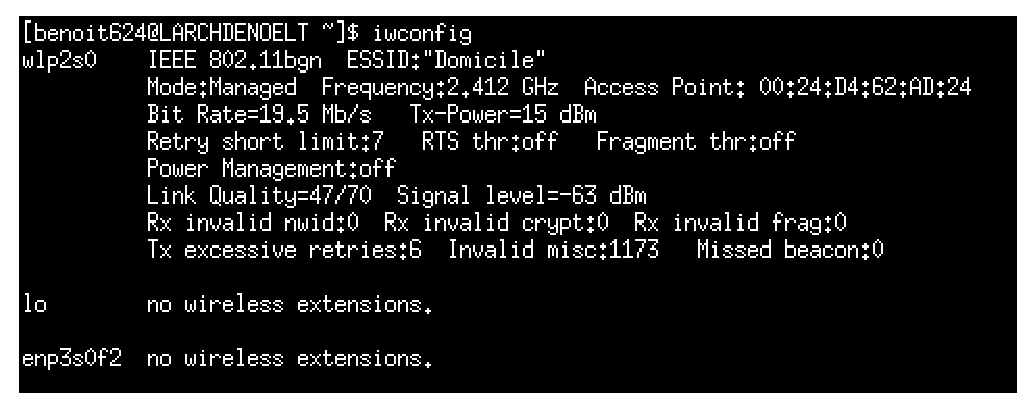
\includegraphics[width=\textwidth]{images/iwconfig}
  \end{figure}
  puis taper:\\
  \begin{lstlisting}
    wifi-menu -o  #votre carte reseaux ou
    wifi-menu
  \end{lstlisting}
  
  \begin{figure}[h]
    \includegraphics[width=\textwidth]{images/wifi-menu}
  \end{figure}
  \chapter{telechargement des package de base}
  Nous allons commencer par telecharger sur /mnt soit / les package de base et de
  base pour developper\\
  \begin{lstlisting}
    pacstrap /mnt base base-devel
  \end{lstlisting}
  
  \begin{figure}[h]
    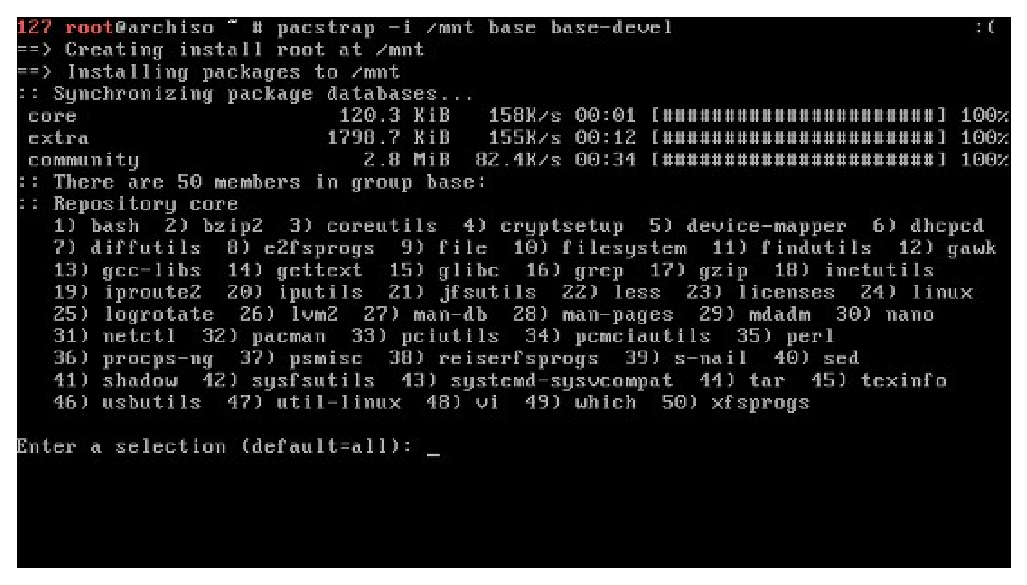
\includegraphics[width=\textwidth]{images/pacstrapbase}
  \end{figure}
  \section{package internet}
  ensuite vous aurez besoin de vous connecter à internet il est donc obligatoire
  d'installer ce packet\\
  \begin{lstlisting}
    pactrap /mnt networkmanager
  \end{lstlisting}
  
  \pagebreak
  \section{packet optionnel}
  Si vous souhaiter un éditeur de texte les deux principaux et
  puissant qui vous seront presenter seront Vim ou Emacs\@:\\
  \begin{lstlisting}
    pacstrap /mnt vim
    pacstrap /mnt emacs
  \end{lstlisting}
  Ensuite vous pouvez installer \textbf{alsamixer} pour pouvoir gerez le son de
  votre machine\@:\\
  \begin{lstlisting}
    pacstrap /mnt alsa-utils
  \end{lstlisting}
  Ensuite pour vous en servir il suffit d'executer\@:
  \begin{lstlisting}
    alsamixer
  \end{lstlisting}
  \begin{figure}[h]
    \includegraphics[width=\textwidth]{images/Alsamixer}
  \end{figure}

  Il existe aussi un outil pour manipuler les log de votre machine\@:\\
  \begin{lstlisting}
    pacstrap /mnt syslog-ng
  \end{lstlisting}
  Pour avoir l'heure regler vous devrez avoir \textbf{ntpd} d'installer\@:\\
  \begin{lstlisting}
    pacstrap /mnt ntpd
  \end{lstlisting}
  Enfin pour pour zipper et dezipper vous pouvez utiliser\@:\\
  \begin{lstlisting}
    pacstrap /mnt zip unzip p7zip
  \end{lstlisting}
  Et enfin si vous êtes en dualboot avec windows vous pourrez manipuler tout vos
  dossier et fichier avec\@:\\
  \begin{lstlisting}
    pacstrap /mnt mtools dosfstools ntfs-3g
  \end{lstlisting}
  Pour vous déplacer plus facilement dans vos dossier vous pouvez utiliser
  \textbf{mc}\\
  \begin{lstlisting}
    pactrap /mnt mc
  \end{lstlisting}
  
  \begin{figure}[h]
    \includegraphics[width=\textwidth]{images/mc}
  \end{figure}
  
  \section{Fstab}
  On peut maintenant generer le fichier fstab qui contient les information sur
  l'architecture de votre archlinux\\
  \begin{lstlisting}
    genfstab -Up /mnt >> /mnt/etc/fstab
  \end{lstlisting}
  
  \begin{figure}[h]
    \includegraphics[width=\textwidth]{images/fstab}
  \end{figure}
  Vous pourrez le modifiez plus tard pour par exemple monter une partition
  Windows au démarrage\@:\\
  \begin{lstlisting}
    UUID=UUID filesystem mountpoint ntfs-3g user, rw, relatime, data=ordered 0 2
  \end{lstlisting}
  
  \chapter{Bootloader}
  \section{Installation en Monoboot}
  Nous allons ici utiliser syslinux un outil puissant et repide pour booter sur
  seulement un OS.
  \begin{figure}[h]
    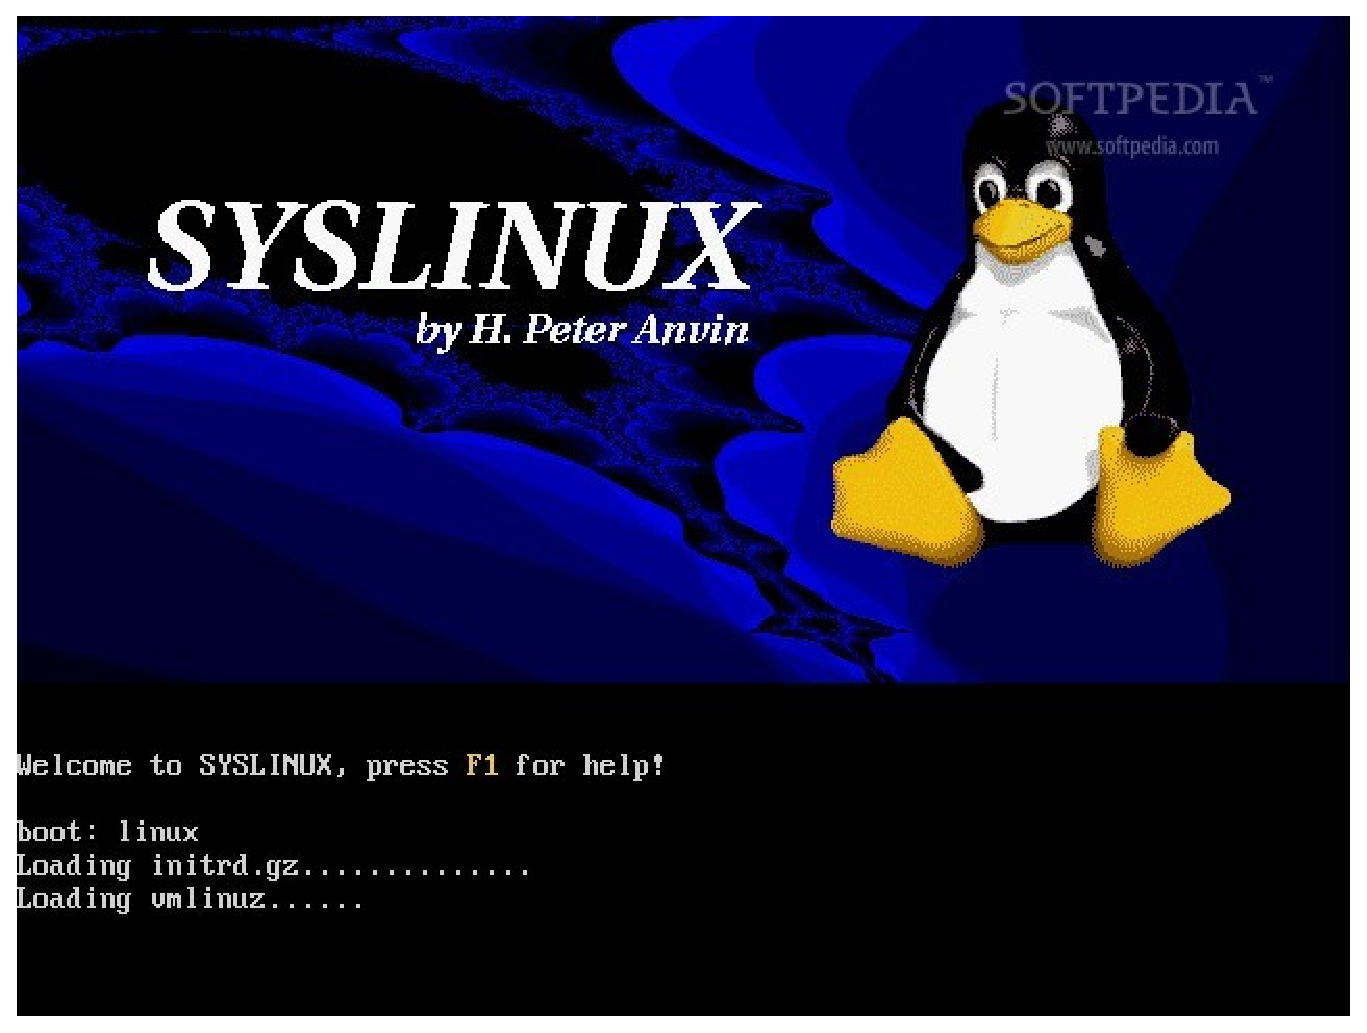
\includegraphics[width=\textwidth]{images/syslinux}
  \end{figure}
  Ainsi pour commecer on va l'installer grace à cette commande\@:\\
  \begin{lstlisting}
    pacstrap /mnt syslinux
  \end{lstlisting}
  Ensuite vous pouvez faire une installation automatique de Linux mais avant cela
  vous aurez besoin de savoir si vos partitions sont en gpt ou mbr\@:\\
  \begin{lstlisting}
    parted -l /dev/ref
  \end{lstlisting}
  Pour les UEFI vous devrez:
  \begin{lstlisting}
    pacstrap /mnt syslinux dosfstools efibootmgr
  \end{lstlisting}
  Pour les autres\@:
  Ensuite en fonction vous lancerez l'installation avec\@:\\
  \begin{lstlisting}
    # Pour les GPT
    pacstrap /mnt gptfdisk
    arch-chroot /mnt
    syslinux-install_update -ia
    
    # Pour les MBR
    arch-chroot /mnt
    syslinux-install_update -iam
  \end{lstlisting}
  Et voila c'est fini, mais si vous voulez le personalis\'e referrer vous à\\
  \url{https://wiki.archlinux.org/index.php/Syslinux}
  \section{Installation pour dualboot}
  Nous allons ici utiliser Grub un des systeme pour gerer deux OS\@:\\
  \begin{figure}[h]
    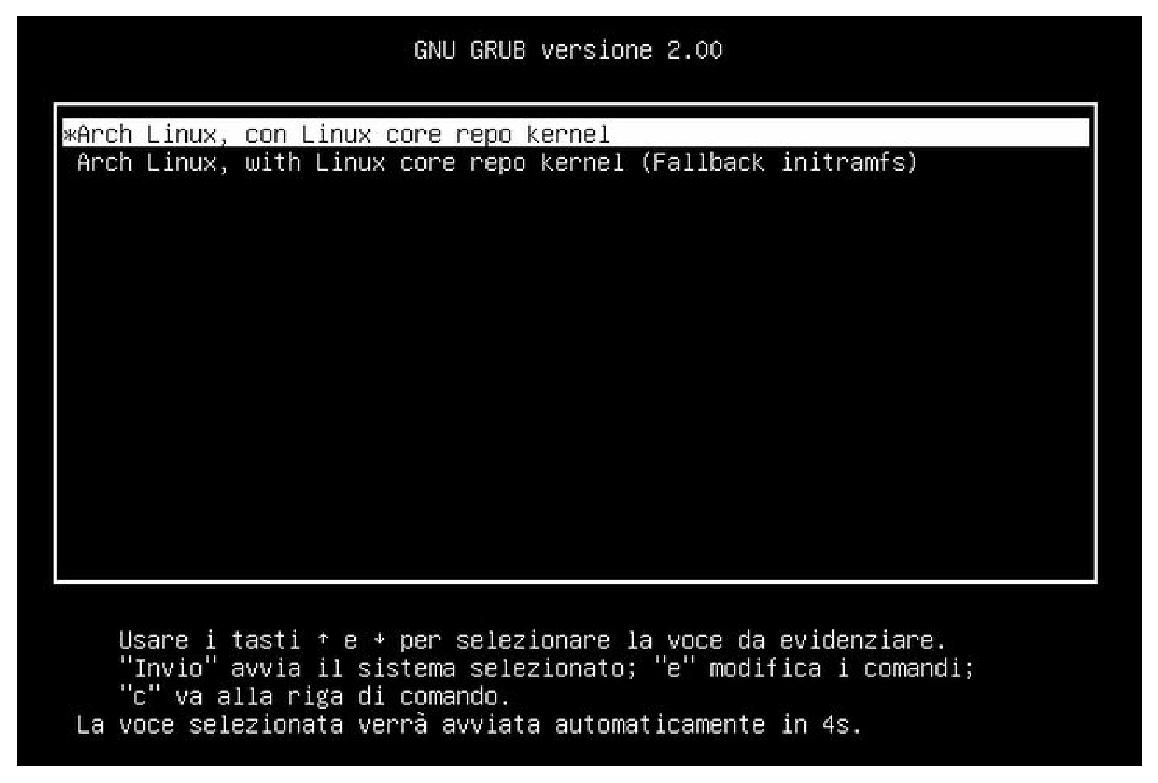
\includegraphics[width=\textwidth]{images/grub}
  \end{figure}
  Commençons par installer les packet necessaire\@:\\
  \begin{lstlisting}
    pacstrap /mnt grub os-prober efibootmgr  #efibootmgr est surtout pour les 
    uefi
  \end{lstlisting}
  Nous allons maintenant booter sur notre Archlinux\@:\\
  \begin{lstlisting}
    arch-chroot /mnt
  \end{lstlisting}
  Et finir l'installation de GRUB\\
  \begin{lstlisting}
    mkinitcpio -p linux
    grub-mkconfig -o /boot/grub/grub.cfg
  \end{lstlisting}
  Pour une installation en BIOS\@:\\
  \begin{lstlisting}
    grub-install --no-floppy --recheck /dev/ref
  \end{lstlisting}
  Pour une installation UEFI\@:\\
  \begin{lstlisting}
    grub-install --target=x86_64-efi --efi-directory=/boot/efi
    --bootloader-id=arch\_grub --recheck
  \end{lstlisting}
  %\section{PXE}
  \chapter{Configuration de la langue}
  Pour avoir le clavier dans la bonne langue il faut se referer \ldots
  pour le clavier francais if faut ecrire dans \textbf{/etc/vconsole.conf}
  \\
  \begin{lstlisting}
    KEYMAP=fr-latin9
    FONT=lat9w-16
  \end{lstlisting}
  Pour la localite francaise\@:\\
  \begin{lstlisting}
    Dans /etc/locale.conf
    LANG=fr_FR.UTF-8
    LC_COLLATE=C
    decommenter fr_FR.UTF8 UTF8 dans /etc/locale.gen
    locale-gen
  \end{lstlisting}
  Enfin pour avoir avoir le fuseau horaire il vous faut cree ce lien\@:\\
  \begin{lstlisting}
    ln -sf /usr/share/zoneinfo/Europe/Paris /etc/localtime
    hwclock --systoch --utc # seulement si vous etes en monoboot
  \end{lstlisting}
  \chapter{Activation des système au démarrage}
  Activation de la connection au reseaux automatiquement\@:\\
  \begin{lstlisting}
    systemctl enable NetworkManager
  \end{lstlisting}
  Activation de la synchronisation des de l'horloge\@:\\
  \begin{lstlisting}
    systemctl enable ntpd
  \end{lstlisting}
  Activation du  generateur de log\\
  \begin{lstlisting}
    systemctl enable syslog-ng
  \end{lstlisting}
  et d'autres precedement explique\@:\\
  \begin{lstlisting}
    systemctl enable cronie
    systemctl enable avahi-daemon
    systemctl enable avahi-dnsconfd
    systemctl enable bluetooth #que pour les appareil bluetooth
  \end{lstlisting}
  \chapter{personalisation de votre machine}
  Pour lui donner un nom editer \textbf{/etc/hostname}\\
  \begin{lstlisting}
    Le_nom_de_votre_machine
  \end{lstlisting}
  Il est aussi conseiller de mettre un mot de passe pour le super user ``root''
  avec cette commande\@:\\
  \begin{lstlisting}
    passwd root
    Enter new UNIX password:
    Retype new Unix password:
    passwd: password updated successfully
  \end{lstlisting}
  Enfin a fin d'avoir YAOURT\footnote{Yaourt est un programme en ligne de 
    commande qui interface les fonctions de pacman et makepkg pour la gestion 
  des paquets sous Arch Linux.} nous allons ajouter au fichier
  \textbf{/etc/pacman.conf}\\
  \begin{lstlisting}
    [archlinuxfr]
    SigLevel = Optional TrustAll
    Server = http://repo.archlinux.fr/$arch
  \end{lstlisting}
  et si vous voulez installer des logiciel uniquement disponible en 32 bits enlever les \#
  dans ce même fichier\@:\\
  \begin{lstlisting}
    #[multilib]
    #Include = /etc/pacman.d/mirrorlist
  \end{lstlisting}
  Si vous voulez encore plus de personalisation vous pouvez ajouter\@:\\
  \begin{lstlisting}
    ILoveCandy
  \end{lstlisting}
  pour avoir une barre de chargement en forme de pacman ou encore\@:\\
  \begin{lstlisting}
    Color
  \end{lstlisting}
  pour avoir pacman en couleur.\\
  Ensuite pour installer le fameux yaourt synchronise puis installer avec les
  commande suivante\@:\\
  \begin{lstlisting}
    pacman -Syu
    pacman -S yaourt
  \end{lstlisting}
  Enfin vous pouver quitter votre session, demonter votre archlinux et relancer
  votre machine\@:\\
  \begin{lstlisting}
    exit
    umount -R /mnt
    reboot
  \end{lstlisting}
  Si tout c'est bien passer vous allez demarrer votre Archlinux.
  Commencer par synchroniser et rafraichir les packets de pacman\@:\\
  \begin{lstlisting}
    pacman -Syy
  \end{lstlisting}
  Et maintenant vous pouvez installer yaourt
  Maintenant vous serais surement heureux d'apprendre a cree un utilisateur.
  Je vais commence par vous presenter une utilisation courante de useradd\@:\\
  \begin{lstlisting}
    useradd -m -g users -G wheel -c 'comment' -s /bin/bash name -p password
  \end{lstlisting}
  Décortiquons ce charabia à present\@:
  \begin{enumerate}
    \item -m creation du repertoire home
    \item -g groupe principal
    \item -G groupe supplementaire \'wheel\' utile pour utiliser sudo
    \item -c le comentaire \' nom principal de l'utilisateur
    \item -s le shell utilise.
    \item -p initialisation du mot de passe
  \end{enumerate}
  Comme je vous explique plus haut nous allons configurer sudo\footnote{est un
    programme conçu pour permettre à un administrateur système de déléguer des
    privilèges à des utilisateurs, et ainsi leur permettre de lancer certaines
    (ou toutes) commandes en tant que root ou autre utilisateur tout en
  enregistrant l'utilisation de ces privilèges.}
  pour cela vous aller taper la commande \textbf{visudo}
  et décommenter la ligne suivante\@:\\
  \begin{lstlisting}
    #wheel ALL=(ALL) ALL
  \end{lstlisting}
  \part{Archlinux en graphique}
  \chapter{Xorg}
  Afin de pouvoir interagir graphiquement avec votre machine vous devrez
  utiliser Xorg
  \section{Definition}
  X.org est l'implémentation officielle du système graphique X Window System 
  dirigée par la X.Org Foundation. Elle est libre et open source. Le système X 
  Window prend en charge l'interface graphique sous GNU/Linux, et vous sera donc
  indispensable si vous souhaitez autre chose que les ttys sur votre Archlinux!
  \\
  Xorg seul est limité (il ne sait qu'afficher des fenêtres), il vous faudra un 
  gestionnaire de fenêtres ou un environnement de bureau complet à lancer dedans.
  \\
  Ces derniers s'installent via pacman et sont soit démarrés directement avec 
  startx soit par l’intermédiaire d’un gestionnaire de connexion graphique. 
  (GDM, KDM, Slim, etc)
  \section{Les g\'enereaux}
  Pour commencer il y a les obligatoire\@:\\
  \begin{lstlisting}
    pacman -S xorg-server xorg-xinit xorg-xmessage xorg-utils xorg-server-utils
    xorg-apps
  \end{lstlisting}
  ensuite pour la souris et le clavier ils sont installable de cette façon\@:\\
  \begin{lstlisting}
    pacman -S xf86-input-mouse xf86-input-keyboard
  \end{lstlisting}
  \section{bonus}
  Et pour ce qui on un clavier tactile ils sera necessaire d'installer\@:\\
  \begin{lstlisting}
    pacman -S xf86-input-synaptics
  \end{lstlisting}
  \section{pilote video}
  Pour les pilote video vous aurez besoin de vous referez au lien suivant\@:
  \url{https://wiki.archlinux.fr/Xorg#Pilotes_libres}
  \chapter{Login Manager}
  %\section{Console}
  \section{graphical}
  \subsection{GDM}
  GDM est un des loggings manager les plus connu facile à installer et pratique
  il comblera vos attente.
  Ensuite pour le démarrer il suffira d'utiliser cette commande\@:\\
  \begin{lstlisting}
    systemctl start gdm.service
  \end{lstlisting}
  \chapter{Interface Graphique}
  Maintenant que votre login manager est install rien de plus simple pour
  installer votre interface graphique.
  \section{Gnome}
   GNOME (prononciation gah-nohm ou nohm) est un environement graphique qui a
   pour but d'etre simple d'utilisation. GNOME fait parti du GNU Project.
  \begin{lstlisting}
    pacman -S gnome gnome-extra
  \end{lstlisting}
  \section{I3}
  i3 est un ``dynamic tiling window manager'' inspir de wmii il est beaucoup
  plus compliqu\'e a utilis\'e que GNOME.\\
  I3 poss\'e une très bonne documentation.% multi-monitor support, a tree structure for windows, and different modes like in vim.
  %\chapter{Utilitaire}
  %\section{nmap}

%\backmatter
  \end{document}
